\documentclass{article}
\usepackage[utf8]{inputenc}
\usepackage{graphicx}
\usepackage{sectsty}

\title{Final Sheet}
\author{}
\date{December 2021}
\renewcommand\thesubsection{\thesection.\alph{subsection}}
\subsectionfont{\fontsize{11}{15}\normalfont}
\renewcommand{\theenumi}{\roman{enumi}}
\usepackage[margin=1in]{geometry}
\begin{document}

\maketitle

\section{Data}

\subsection{Types of Variables}

\textbf{Qualitative/Categorical}
\begin{itemize}
    \item Outcomes fall into different categories
    \item Categories can be ordered
\end{itemize}

\noindent
\textbf{Quantitative}
\begin{itemize}
    \item Measured on a numeric scale
\end{itemize}

\subsection{Summarizing Data Visually}

\textbf{Qualitative/Categorical Data}
\begin{itemize}
    \item Frequency tables - displays all categories of a single categorical variable with associated frequencies 
    \item Contingency tables - display two categorical variables simultaneously
    \item Marginal distributions - display distribution of one of the two variables only
    \item Conditional distributions - display distribution of one variable, satisfying a condition of the other variable
    \item Bar charts
    \item Pie charts
\end{itemize}

\noindent
\textbf{Quantitative Data}
\begin{itemize}
    \item \textbf{Graphically}
    \begin{itemize}
        \item Histogram
        \item Stem-and-leaf displays
        \item Boxplots
    \end{itemize}
    \item \textbf{Shape of the Distribution}
    \begin{itemize}
        \item Modality (number of peaks):
        \begin{itemize}
            \item unimodal
            \item bimodal
            \item multimodal
        \end{itemize}
        \item Symmetry of distribution:
        \begin{itemize}
            \item unimodal
            \item skewed to right (long right tail)
            \item skewed to left (long left tail)
        \end{itemize}
        \item Presence of outliers 
    \end{itemize}
    \item \textbf{Numerically}
    \begin{itemize}
        \item Measures of center: 
        \begin{itemize}
            \item mean
            \item median
        \end{itemize}
        \item Measures of spread: 
        \begin{itemize}
            \item variance: \begin{math}s^2 = \frac{\Sigma_{i=1}^{n}(y_1 - \overline{y})^2}{n-1}\end{math}
            \item standard deviation: \begin{math}s = \sqrt{\frac{\Sigma_{i=1}^{n}(y_1 -\overline{y})^2}{n-1}}\end{math}
            \item interquartile range \begin{math}IQR = Q3 - Q1\end{math}
        \end{itemize}
        \item Percentiles (also called quantiles)
        \item 5-number summary:
        \begin{itemize}
            \item minimum
            \item first quartile (Q1)
            \item second quartile (Q2)
            \item third quartile (Q3)
            \item maximum
        \end{itemize}
    \end{itemize}
    \item \textbf{Sensitivity to Outliers}
    \begin{itemize}
        \item Sensitive to outliers:
        \begin{itemize}
            \item mean
            \item range, variance, standard deviation
        \end{itemize}
        \item Not sensitive to outliers
        \begin{itemize}
            \item median
            \item IQR
        \end{itemize}
    \end{itemize}

\end{itemize}

\section{Normal Distribution}

\textbf{Characteristics of the Normal Model}
\begin{itemize}
    \item bell-shaped; unimodal
    \item perfectly symmetric about the mean
    \item spread of distribution determined by value of standard deviation
    \item mean \begin{math}\mu\end{math} and the standard deviation \begin{math}\sigma\end{math} are parameters(numerical characteristics of a model)
    \item mean \begin{math}\overline{y}\end{math} and standard deviation \emph{s} are statistics (numerical characteristics of a sample)
\end{itemize}

\noindent
\textbf{The 68-95-99.7 Rule}
\begin{itemize}
    \item 68\% of data falls within 1 \begin{math}\sigma\end{math} of \begin{math}\mu\end{math} 
    \item 95\% of data falls within 2 \begin{math}\sigma\end{math} of \begin{math}\mu\end{math} 
    \item 99.7\% of data falls within 3 \begin{math}\sigma\end{math} of \begin{math}\mu\end{math} 
\end{itemize}

\noindent
\textbf{Finding Areas Under the Normal Model}\\\\
\textbf{Algorithm}
\begin{itemize}
    \item Identify the: \\
    \begin{math}\mu\end{math} - mean of the model \\
    \begin{math}\sigma\end{math} - standard deviation of the model \\
    \emph{y} - observed value
    \item Construct the normal model: N(\begin{math}\mu\end{math},\begin{math}\sigma\end{math})
    \item Calculate the z-score (z): \begin{math}z = \frac{\emph{y} - \mu}{\sigma}\end{math}
    \item Using R compute the p-value:
    \begin{itemize}
        \item Area below \emph{y}: pnorm(\emph{z})
        \item Area above \emph{y}: pnorm(\emph{z} , lower.tail = F)
        \item Area in between \begin{math}\emph{y}_1\end{math} and \begin{math}\emph{y}_2\end{math} (where \begin{math}\emph{y}_1\end{math} $>$ \begin{math}\emph{y}_2\end{math}): pnorm(\begin{math}z_1\end{math}) - pnorm(\begin{math}z_2\end{math})
    \end{itemize}
    \item \textbf{Finding Z-Score from the Area Under the Normal Model}
    \begin{itemize}
        \item Area above unknown \emph{y}: qnorm(\emph{p}, lower.tail = F)
        \item Area below unknown \emph{y}: qnorm(\emph{p})
    \end{itemize}
\end{itemize}

\section{Binomial Distribution}

\section{Correlation and Association}

\textbf{Scatterplots}
\begin{itemize}
    \item Direction:
    \begin{itemize}
        \item Positive (\emph{x} and \emph(y) values tend to go in the same direction)
        \item Negative (\emph{x} and \emph{y} values tend to go in the opposite direction)
    \end{itemize}
    \item Form:
    \begin{itemize}
        \item Linear
        \item Non-linear
    \end{itemize}
    \item Point relationship:
    \begin{itemize}
        \item Strong relationship between points
        \item weak or no relationship between points (randomly scattered)
    \end{itemize}
    \item Outliers
\end{itemize}

\noindent
\textbf{Correlation (\emph{r})}
\begin{itemize}
    \item Positive correlation: large \emph{x} values are linearly associated with large \emph{y} values (\emph{r} is positive)
    \item Negative correlation: large \emph{x} values are linearly associated with small \emph{y} values (\emph{r} is negative)
    \item \emph{r} has a value between 1 and -1, and has no units
    \item \begin{math}
    r = \frac{\Sigma z_x * z_y}{n - 1}
    \end{math}
\end{itemize}

\noindent
\textbf{Association vs Causality}
\begin{itemize}
    \item Association does not imply causation. There may be a lurking variable
\end{itemize}

\section{Regression Analysis}

\textbf{The Regression Line}
\begin{itemize}
    \item Equation for regression line: \begin{math}\hat y = intercept + (slope * x)\end{math}
    \item Equation for slope: \begin{math}
    slope = r * \frac{s_y}{s_x}
    \end{math}\\
    (where \begin{math}s_y\end{math} and \begin{math}s_x\end{math} are the standard deviations of y and x respectively)
    \item Equation for intercept: \begin{math}
    intercept = \overline{y} - (slope * \overline{x})
    \end{math} \\
    (where \begin{math}\overline{y}\end{math} and \begin{math}\overline{x}\end{math} are the mean y and x values respectively)
\end{itemize}

\noindent
\textbf{The Residuals}
\begin{itemize}
    \item The residual (\emph{e}) is the difference between observed value \emph{y} and the predicted value \begin{math}
    \hat{y}
    \end{math}. Therefore:\\
    \emph{e} = \emph{y} (from data) - \begin{math}
    \hat{y}
    \end{math} (from model)
    \item The sum of residuals is equal to zero
    \item Linear model is obtained by minimizing the sum of the squared residuals. Therefore, also referred to as the least squares regression line
    \item To assess appropriateness of regression model, we use the residual plot (plots residuals against explanatory variable data). If plot shows no pattern, model is appropriate. 
\end{itemize}

\section{Experiments and Observational Studies}

\textbf{Types of Studies}
\begin{itemize}
    \item Observational Studies
    \begin{itemize}
        \item Investigators have no control over either variable
        \item No deliberate human intervention 
        \item Retrospective study: based on information from events that have taken place in the past
        \item Prospective study: data and information is gathered in real time
    \end{itemize}
    \item Experiments 
    \begin{itemize}
        \item Involves planned intervention on the exposure to a condition suspected of altering the response outcome
        \item Most often control group(s) will be used
    \end{itemize}
\end{itemize}

\noindent
\textbf{Randomized, Comparative Experiments}
\begin{itemize}
    \item Involves assessing the effect of an explanatory variable, called a factor, on a response variable
    \item Compares the response variable between different levels of the factor
    \item Experimenters control what type of treatment individuals receive, the treatment assignment is random
    \item Participants referred to as subjects or experimental units
    \item The treatment a subject receives will be a combination of the levels from different factors 
\end{itemize}

\noindent
\textbf{Principles of Experimental Design}
\begin{itemize}
    \item Randomize
    \begin{itemize}
        \item Treatments are randomly assigned to subjects
    \end{itemize}
    \item Replicate
    \begin{itemize}
        \item Comparison between different treatment groups will not be reliable unless more individuals receive each treatment 
    \end{itemize}
    \item Blocking
    \begin{itemize}
        \item May be beneficial to control for variables that are not factors but are believed to have some influence on the response variable 
        \item Subjects are divided into blocks (ex. male and female groups). Treatment assignment and comparisons are done within each block separately 
    \end{itemize}
\end{itemize}

\noindent
\textbf{Blinding and Placebo}
\begin{itemize}
    \item Single Blind: either the subjects or the evaluators are blinded as to treatment assignment
    \item Double Blind: neither the subjects nor the evaluators knows the treatment assignments
    \item Blinding is usually done using a placebo which is designed to look like the treatment but has no real treatment value
\end{itemize}

\section{Types of Sampling}

\textbf{Sampling Methods}
\begin{itemize}
    \item Simple Random Sampling
    \begin{itemize}
        \item Consists of \emph{n} individuals sampled at random from the population
        \item Each individual has an equal chance of being selected
        \item Each possible sample size \emph{n} is equally likely
    \end{itemize}
    \item Stratified Sampling
    \begin{itemize}
        \item Population is divided into strata (a stratum is a subset of the population that shares a particular characteristic)
        \item Simple random sample is drawn from each stratum
        \item Stratified sample has smaller variability across samples and hence give more reliable results 
    \end{itemize}
    \item Cluster Sampling
    \begin{itemize}
        \item Can be used when natural groups in a population exist
        \item Population is divided into those groups/clusters
        \item Simple random sample from all clusters is obtained
        \item If all individuals in a selected cluster are included, final sample is a one-stage cluster sample
        \item If additional simple random sample is drawn from selected clusters, final sample is a two-stage cluster sample
        \item This method is used for the sake of convenience, practicality, and cost-efficiency
    \end{itemize}
    \item Multistage Sampling
    \begin{itemize}
        \item Involves more than one stage or more than one sampling procedure in obtaining a sample
    \end{itemize}
    \item Systematic Sampling
    \begin{itemize}
        \item Obtained by selecting every \emph{k}th individual from the sampling frame
        \item Method can be used as long as list being sampled from does not contain a hidden order
    \end{itemize}
\end{itemize}

\noindent
\textbf{Bad Sampling Procedures and Biases}
\begin{itemize}
    \item Undercoverage
    \begin{itemize}
        \item When sampling frame or sampling procedure excludes or under-represents certain types of individuals from the population 
    \end{itemize}
    \item Convenience Sampling
    \begin{itemize}
        \item Selecting individuals from a population based on availability and access
    \end{itemize}
    \item Voluntary Response Bias
    \begin{itemize}
        \item If responses are voluntary, those with strong opinions tend to be over-represented 
    \end{itemize}
    \item Non-response Bias
    \begin{itemize}
        \item Individuals who do not respond in a survey might differ from the respondents in certain aspects
        \item Including only the respondents in a sample will result in non-response bias
    \end{itemize}
    \item Response Bias
    \begin{itemize}
        \item Subject's response is influenced by how the question was phrased or asked, or due to misunderstanding of a question, or unwillingness to disclose the truth 
    \end{itemize}
\end{itemize}

\section{Hypothesis Testing}
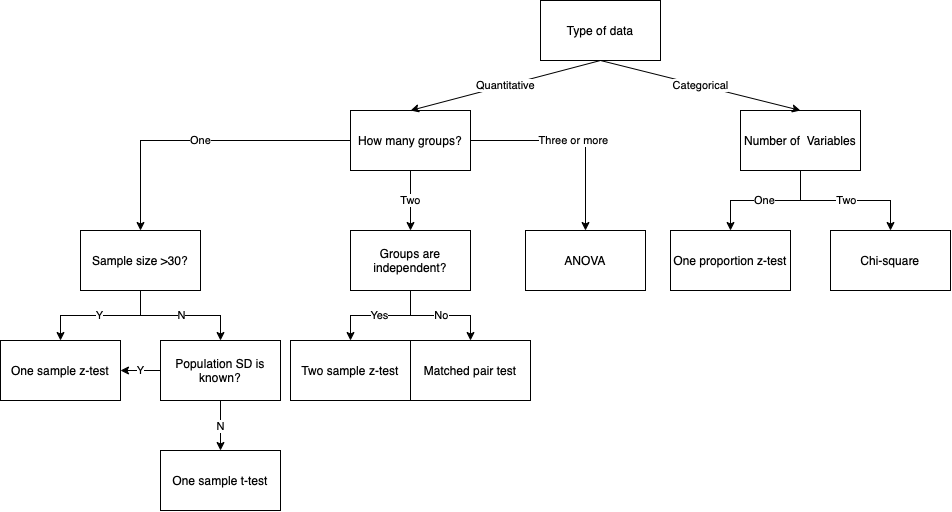
\includegraphics[scale = 0.5]{dec-tree.png}
\subsection{One sample z-test}
\textbf{Algorithm}
\begin{itemize}
\item Idenitify parameter of interest. Find the null and alternative hypotheseses.\\
      s - The standard deviation of the sample.\\
      n - The sample size.\\
      $\mu$ - Hypothethised population mean.\\
      $\mathbf{SE}(\bar{y}) = \frac{s}{\sqrt{n}}$ - Standard error of the statistic.
\item Construct the null-model: $\mathbf{N}(\mu,\frac{s}{\sqrt{n}})$
\item Find the test-statistic(t): $\mathbf{Z} = \frac{x-\mu}{\mathbf{SE}(\bar{y})}$
\item Using R compute the p-value:
\begin{itemize}
    \item One-sided hypothesis : pnorm(t)
    \item Two-sided hypothesis : 2 $\cdot$ pnorm(t)
\end{itemize}
\item If the p-value is less than $\alpha$ - reject the null-hypothesis. 
    Otherwise, you fail to reject the null-hypothesis.
\end{itemize}
\subsection{One proportion z-test}
\textbf{Algorithm}
\begin{itemize}
\item Idenitify parameter of interest. Find the null and alternative hypotheseses.\\
      n - The sample size.\\
      $p_0$ - Hypothethised proportion.\\
      $\mathbf{SD} = \sqrt{\frac{p_0(1-p_0)}{n}}$ - Standard error of the statistic.
\item Construct the null-model: $\mathbf{N}(p_0,\sqrt{\frac{p_0(1-p_0)}{n}})$
\item Find the test-statistic(t): $\mathbf{Z} = \frac{x-p_0}{\mathbf{SD}}$
\item Using R compute the p-value:
\begin{itemize}
    \item One-sided hypothesis : pnorm(t)
    \item Two-sided hypothesis : 2 $\cdot$ pnorm(t)
\end{itemize}
\item If the p-value is less than $\alpha$ - reject the null-hypothesis. 
    Otherwise, you fail to reject the null-hypothesis.
\end{itemize}
\subsection{Two sample z-test}
\textbf{Algorithm}
\begin{itemize}
\item Idenitify parameter of interest. Find the null and alternative hypotheseses.\\
      s - The standard deviation of the sample.\\
      n - The sample size.\\
      $\mu$ - Hypothethised population mean.\\
      $\mathbf{SD}(\bar{y_1}-\bar{y_2}) = \sqrt{\frac{\sigma_1^2}{n_1}+\frac{\sigma_2^2}{n_2}}$ - Standard error of the statistic.
\item Construct the null-model: $\mathbf{N}(\mu,\frac{s}{\sqrt{n}})$
\item Find the test-statistic(t): $\mathbf{Z} = \frac{x-p_0}{\mathbf{SE}(\bar{y})}$
\item Using R compute the p-value:
\begin{itemize}
    \item One-sided hypothesis : pnorm(t)
    \item Two-sided hypothesis : 2 $\cdot$ pnorm(t)
\end{itemize}
\item If the p-value is less than $\alpha$ - reject the null-hypothesis. 
    Otherwise, you fail to reject the null-hypothesis.
\end{itemize}
\subsection{Matched pair}
\subsection{One sample t-test}
\subsection{ANOVA}


\end{document}